\chapter*{Úvod}
\addcontentsline{toc}{chapter}{Úvod}

%\section*{Magnetooptické jevy a jejich využití}
Jako první se jevy, kdy látka ovlivňovala šíření světla v závislosti na magnetickém poli, zabýval Faraday. Roku 1845 objevil, že rovina lineárně polarizovaného světla se stáčí při průchodu skleněným válcem v magnetickém poli. To mimo jiné vedlo k potvrzení spojitosti světla a magnetismu. K podobnému závěru došel i Kerr, který však narozdíl od Faradaye nezkoumal průchod, ale odraz světla.

Magnetooptické jevy se dají pozorovat, jak bylo uvedeno výše, buď při průchodu, nebo odrazu, přičemž naším cílem je zkoumání druhého, 
častěji zvaného Kerrova, jevu. Co se týče geometrie, máme na výběr ze tří základních konfigurací. Jedná se o polární, longitudiální a 
transversální. Jejich schéma je znázorněno na obrázku \ref{schema geo}. Jakákoliv jiná poloha vektoru magetizace se dá 
složit z těchto tří příadů. V rámci této práce se budeme zabývat poze polárním Kerrový jevem.

\begin{figure}
\begin{center}
    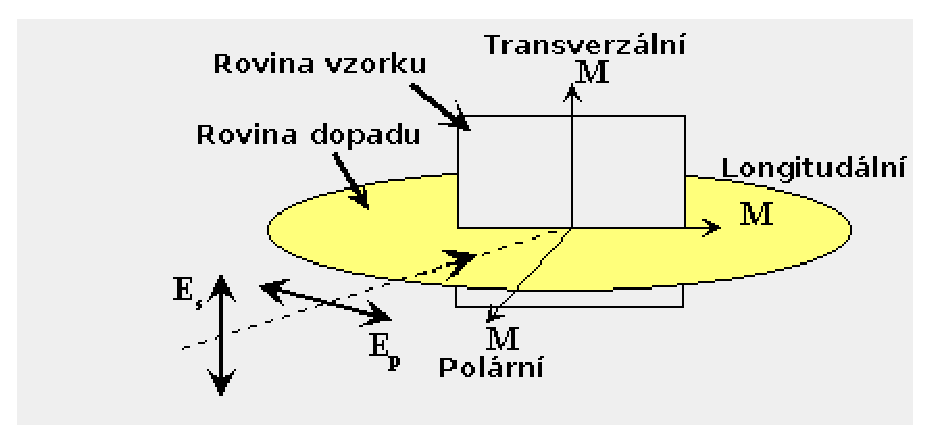
\includegraphics[width=5in]{img/polar.eps}
\end{center}
    \caption{Schéma geometrie Kerrova magnetooptického jevu.}
    \label{schema geo}
\end{figure}

%\section*{Aplikace magnetoopticky}
Experimentální metody využívající magnetooptických jevů jsou hojně využívány ke studiu 
magnetických vlastností materiálů.  Tyto metody se vyznačují vysokou citlivostí, 
selektivní povahou, bezkontaktním snímáním, možností využití časově rozlišených experimentů 
a poměrně rychlou odezvou, která umožňuje měření povrchových hysterezních smyček a pozorování 
magnetických domén. Jsou mimo jiné schopny zprostředkovat důležité informace o profilech 
vrstevnatých systémů a charakteru rozhraní. V tenkých vrstvách je pak možné studovat vliv 
jejich struktury na spinové uspořádání. Kombinace spektroskopické elipsometrie a 
magnetooptické spektroskopie společně s odpovídajícími teoretickými modely poskytuje unikátní 
možnost studia fyzikálních vlastností materiálů ve formě tenkých vrstev s tloušťkami až do 
jednotek nanometrů. Znalost optických a magnetooptických parametrů vyjádřená spektry tenzoru 
dielektrické permitivity dává informaci o elektronové struktuře materiálu a je podstatná 
i pro samotný návrh a optimalizaci funkce integrovaných fotonických prvků.

Mezi další zajímavé aplikace patří 3D displaye využívající magnetické nanovrstvy, jejichž pixely se pohybují pod 1 $\mu$m \cite{3D disp}, 
a magnetooptické izolátory \cite{izolatory}, které propouští světlo pouze jedním směrem. Tyto zařízení jsou nejčastěji používány u výkonných 
laserů, kde zabraňují návratu svazku zpět do laseru.

%\section*{Obsah práce}
Tato práce je zaměřena především na experimentální metody používané k určení magnetooptických veličin. Z tohoto důvodu 
je úvodní kapitola zaměřena na metody popisu polarizovaného světla. Po zavedení základních veličin je podrobně rozebrán Jonesovů formalismus, 
který nám umožňuje nejen popis, ale i určení polarizačního stavu po průchodu optickou soustavou. Tatko kapitola zakončuje zavedením magnetooptických veličin.

V další kapitole je rozebráno šíření světla anizotropním materiálem. Po úvodu do problematiky je stučně popsán formalismus umožňující popis multivrstevnatych 
prostředí a nazávěr je uveden nejednodušší případ pro jednoduchou vrstvu.

Třetí kapitola popisuje dvě experimentální metody užívané pro měření Kerrova jevu. Nejprve je vždy uveden krátký teoretický popis s 
výpočtem, na kterém je založeno samotné měření, a pak následuje zevrubný popis konkrétní aparatury použité v laboratoři. Závěrem je vždy uvedeno pár 
poznámek k ovladacím programům těchto aparatur.

Poslední kapitola se zabývá konkrétnímy výsledky naměřenými na obou aparaturách a jejich porovnáním. Rozebrány jsou tři odlišné skupiny vzorků, 
na kterých jsou ukázány klady a zápory jednotlivých metod. U každého vzorku je také stručná zmínka o jeho užití a způsobu, kterým byl vyroben.
